%%%%%%%%%%%%%%%%%%%%%%%%%%%%%%%%%%%%%%%%%%%%%%%%%%%%%%%%%%%%%%%%%%%%%%%%%%%%%%%%%%%%%%
% TEMPLATE FOR Praktikum P3B
% This template uses the Memoir class. It is a very powerful class for creating documents such
% as reports, papers and theses. You can find more information at CTAN, the Comprehensive
% TeX Archive Network. These is a long manual that describes how to use Memoir.
% https://www.ctan.org/pkg/memoir?lang=en
% Sven Buschke
% Last Update: 2021-08-18
%%%%%%%%%%%%%%%%%%%%%%%%%%%%%%%%%%%%%%%%%%%%%%%%%%%%%%%%%%%%%%%%%%%%%%%%%%%%%%%%%%%%%

%------------------------------------------------------------------------------------
%	EDIT THIS BLOCK
%------------------------------------------------------------------------------------
\newcommand{\studentfullname}{Sven Buschke}			% change to your name
\newcommand{\matrikelnumber}{27205317}				% enter your student number 
\newcommand{\dateexperiment}{24. August 2021}				% change to your partner's name
\newcommand{\timeexperiment}{13:30-18:00 Uhr}				% enter your partner's student number
\title{P3B-Versuch 5C PLW --- Plancksches Wirkungsquantum}					% change to the title of the experiment
\author{\studenfullname}				% you don't have to change this
\date{23.\ August 2021}										% this fills in today's date - don't change



%------------------------------------------------------------------------------------
%	FORMATTING STUFF
%------------------------------------------------------------------------------------

\documentclass[12pt,oneside,oldfontcommands]{memoir}


%-----------------------------------------------------------------------------------
%	MARGIN AND HEADER/FOOTER SIZES
%------------------------------------------------------------------------------------
\setlrmarginsandblock{2.5cm}{2.5cm}{*}  		% left/right margins
\setulmarginsandblock{2.5cm}{2.5cm}{*} 			% top/bottom margins
\checkandfixthelayout							% checks the layout is correct
\setlength{\parindent}{0in}  					% no indent on start of paragraph
							

%-------------------------------------------------------------------------------------
%  PACKAGES
%-------------------------------------------------------------------------------------
\usepackage{amsmath,amsthm,amssymb,amsfonts}			% math fonts
\usepackage[german]{babel}								% hyphenation rules for German
\usepackage{graphicx}									% for importing pdf files 
\usepackage{siunitx}									% si units - extremely useful
\usepackage[usenames,dvipsnames,svgnames,table]{xcolor}	% defines the dvips color names
\usepackage{color,soul} 								% for highlight hi - hyphenation, underlining
%\usepackage{libertine}
%\usepackage{libertinust1math}
%\usepackage[T1]{fontenc}
\usepackage{fontspec}
\usepackage{pdfpages}
\setmainfont{Linux Libertine O}%
   [Ligatures={Common,Historic}, Numbers=OldStyle]
\setulcolor{red} 										% set underline color
\setstcolor{green} 										% set overstriking color
\sethlcolor{green} 										% set highlighting color


%--------------------------------------------------------------------------------------------
%  GRAPHICS PATH
%--------------------------------------------------------------------------------------------
\graphicspath{{figures/}}								% put your figures in a folder called figures



%---------------------------------------------------------------------------
%  SOME NEW FUNCTIONS FOR IMPORTING FIGURES
%---------------------------------------------------------------------------
\newcommand{\placefigure}[1]{\centerline{\includegraphics[width=2 in]{#1}}} 
\newcommand{\placefigureandscale}[2]{\centerline{\includegraphics[width=#2 in]{#1}}} 



%-------------------------------------------------------------------------------------
%	TITLE PAGE MACRO
%------------------------------------------------------------------------------------
\makeatletter
\def\maketitle{%
  \null
  \thispagestyle{empty}
  \begin{center}\leavevmode
       \normalfont

       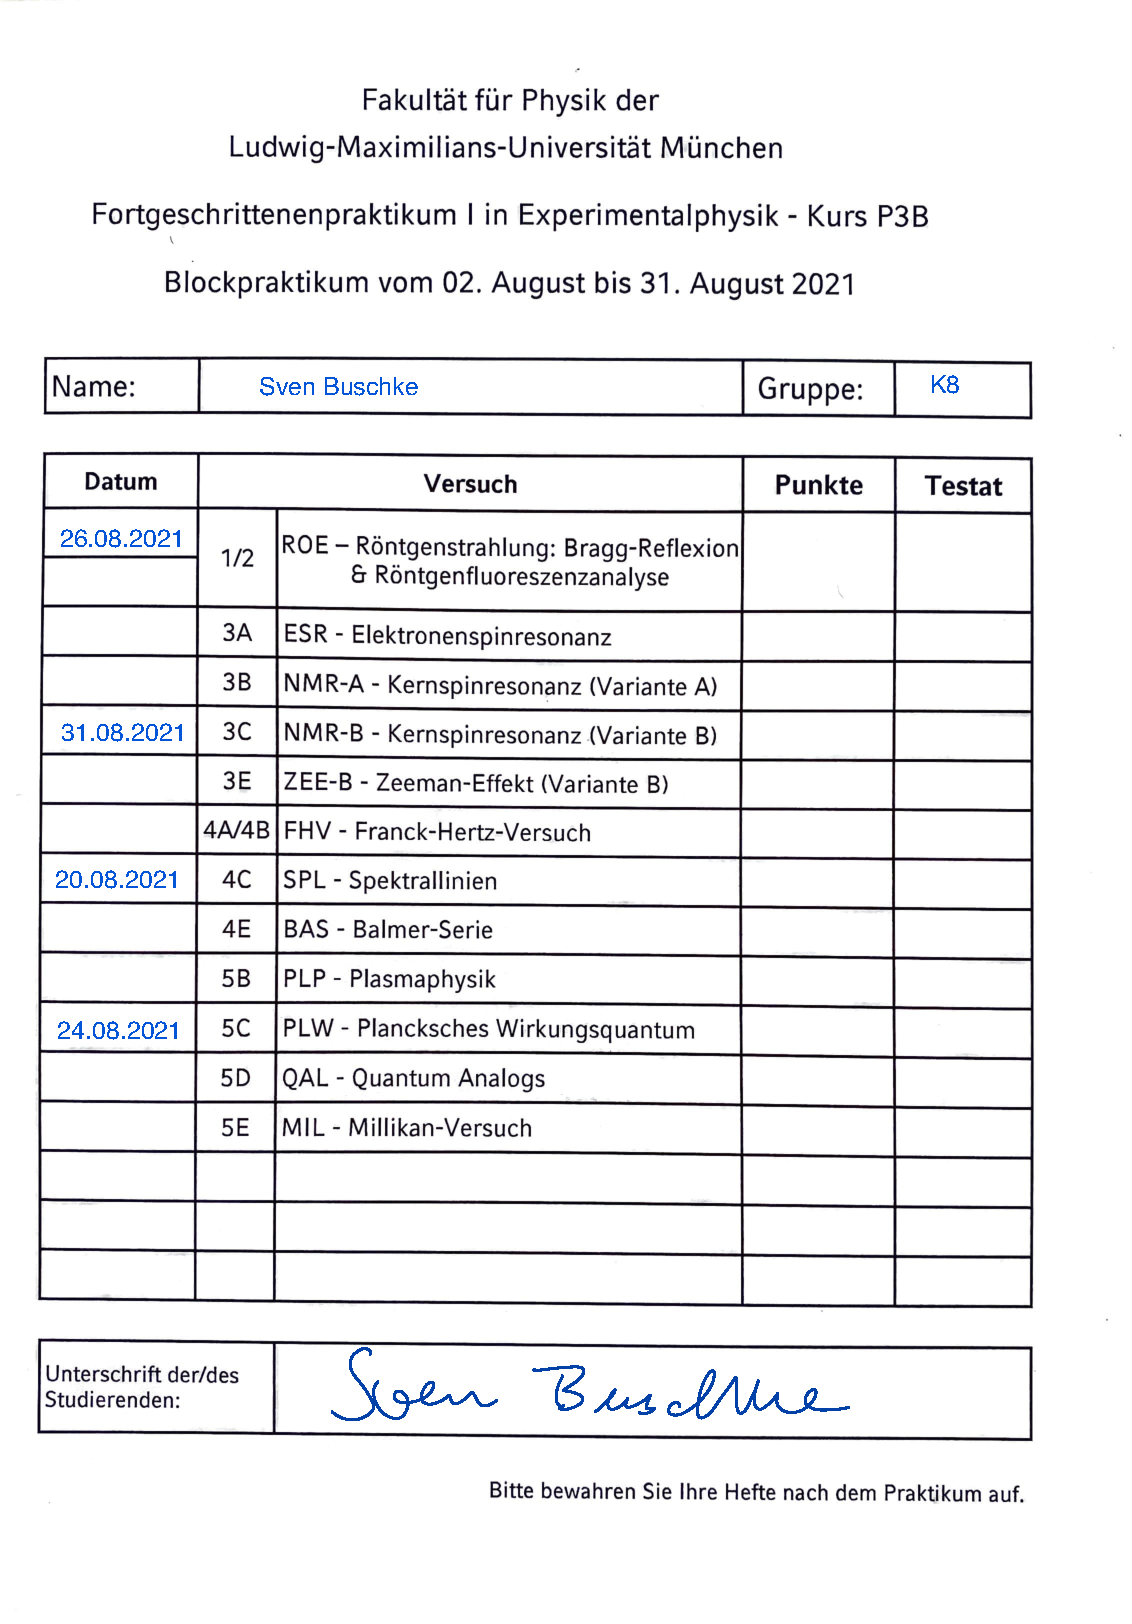
\includepdf[pages=-,scale=0.9,pagecommand={}]{Deckblatt-P3B-signed-20210825.pdf}
       \newpage
       
\includegraphics[width=0.165\columnwidth]{lmu-seal.pdf}
       
\includegraphics[width=0.35\columnwidth]{lmu-logo.pdf}
       \vskip 0.5cm   
       \textsc{\Large P3B-Praktikum}\\[0.5 cm]
	     {\large \@date\par}
       \vskip 1.0cm
	\rule{\linewidth}{0.2 mm} \\[0.4 cm]
	{ \huge \bfseries \@title}\\
	\rule{\linewidth}{0.2 mm} \\[1.5 cm]
	
	\begin{minipage}{0.5\textwidth}
		\begin{flushleft} \large
			\emph{Name:} \studentfullname\\
			Matrikelnummer: \matrikelnumber
			\end{flushleft}
			\end{minipage}~
			\begin{minipage}{0.4\textwidth}
			\begin{flushleft} \large
			Versuchstermin: \dateexperiment\\
			Versuchsdauer: \timeexperiment
		\end{flushleft}
	\end{minipage}\\[2 cm]
   \end{center}
   \vfill
   \null
   \cleardoublepage
  }
\makeatother



%-------------------------------------------------------------------------------------------
%	START OF DOCUMENT
%--------------------------------------------------------------------------------------------

\begin{document}
%\large 
\maketitle
\frontmatter
\let\cleardoublepage\clearpage
\mainmatter
\sloppy



%--------------------------------------------------------------------------------------------
%	RESULTS AND ANALYSIS
%--------------------------------------------------------------------------------------------

\setcounter{tocdepth}{3}
\tableofcontents

\section{Vorbereitung Versuch 5C PLW --- Bestimmung des Planckschen Wirkungsquantums}
\subsection{Physikalische Grundlagen}
Mit diesem Versuch soll das Plancksches Wirkungsquantum auf zweierlei Arten bestimmt werden.
\subsubsection{Stichworte}
\paragraph{Planksches Strahlungsgesetz}
Das Planksche Strahlungsgesetz handelt von der Energiedichte eines idealen Schwarzkörpers. Hierbei legt man die quantisierung der elektromagnetischen Welle zugrunde. $E = \hbar \nu $

Für die Wellenlängen gilt gemäß allgemeinem Strahlungsgesetz:
$S_\lambda(\lambda,T) = \frac{2}{}$
\paragraph{Kontaktspannung}
Die Kontaktspannung ist die Spannung, die entsteht, wenn sich zwei nicht gleiche Materialien berühren. Es gilt: $U_g = \hat{U}_g - U_{kontakt}$
\paragraph{charakteristisches Spektrum}
Das charakteristische Spektrum werden gebildet von charakteristischen Wellenlängen $\lambda$ bei bestimmten Übergängen. Es gilt $E = \hbar \frac{c}{\lambda}$.
\paragraph{Stoßverbreiterung bei Spektrallampen}
Durch Stöße zwischen Atomen werden die Spektrallinien unscharf. Hierdurch kommt es zu Energieverschiebungen, die sich auf die Wellenlänge des emittierten Photons auswirkt und das Spektrum entsprechend verbreitert.
\paragraph{Bändermodell}
Anders als bei einzelnen Atomen kommt es bei Molekülen und noch mehr bei Festkörpern zu weiteren Energieniveaus. Diese lassen sich zu einem Energieband zusammenfassen.

\subsubsection{Theoretischer Hintergrund / Überblick Versuche}
\paragraph{Vorversuch zu Teilversuch 1: Vorversuch Bestimmung des Quecksilberspektrums und der Absoprtionsspektren der Farbfilter}
Im Vorversuch werden die charakteristischen Wellenlängen der Quecksilberlampe und der Xenonlampe bestimmt und die Farbfilter zugeordnet.
\paragraph{Teilversuch 1: Bestimmung des Planckschen Wirkungsquantums mit dem Photoeffekt}
Hier wird mit einer Vakuumphotozelle und Quecksilberdamplampe das Plancksche Wirkungsquantum bestimmmt.
\paragraph{Teilversuch 2: Bestimmung des Planckschen Wirkungsquantums mit Hilfe von Leuchtdioden}
Im Teilversuch wird mit Leuchtdioden das Plancksche Wirkungsquantum durch Messen der Durchlassspannung von LEDs bestimmt.
\section{Versuchsdurchführung und Auswertung}
\subsection{Teilversuch 1: Bestimmung des Planckschen Wirkungsquantums mit dem Photoeffekt mit Vorversuch Bestimmung des Quecksilberspektrums und der Absoprtionsspektren der Farbfilter}
\subsubsection{Versuchsvorbereitung, Grundlagen des Versuches, Erläuterung verwendeter Formelzeichen, Versuchsziel, Erläuterung der Messmethoden, schematische Skizzen, Planung der Durchführung, Versuchsplanung, Versuchsdurchführung}
Versuchsaufbau\\
Das Licht der Quecksilberdampflampe fällt auf den Eingang der Glasfaser. Hier nehmen wir das Quecksilberspektrum auf und bestimmen die Wellenlänge. Gleiches mit der Xenondampflampe.
Nun wird die Photozelle verwendet mit zwei Blendeinstellungen B1 zum Einstellen des Strahldruchmessers und B2 der Lichtintensität. Unter Verwendung von Widerstand R, Erdung verbunden mit der Masses des Cassys zur Vermeidung von Störungen, werden verschiedene Spannungen (-3V bis +3V) angelegt und mit dem Sensor-Cassey gemessen.
Wir nehmen die U-I-Kennlinine auf (Hg-Linie) und bestimmen im linearen Bereich des U-I-Diagramms die Schnittpunkte der Geraden mit der U2-Achse, mit Verwendung einer Ausgleichsgerade.


\subsubsection{Versuchsergebnisse und -auswertung}
Nachfolgend sieht man die graphische Bestimmung des Planckschen Wirkungsquantums aus den Wertepaaren $(U_g,\nu)$:\\

Hier sind noch die Python-Diagramme einzufügen (muss noch nachgeliefert werden).

Die Dioden beginnen zu leuchten, wenn die Schwellenspannung erreicht ist. 
Die Methode führt zu recht eindeutigen Ergebnissen. Der Fehler liegt hierbei im Bereich plus minus .

Gemäß Gaußscher Unsicherheit $\frac{\Delta G}{G} = \sqrt{(a\frac{\Delta x}{x})^2 + (b \frac{\Delta y}{y})^2}$ liegt eine Messunsicherheit vor wie folgt:
Messbreite liegt bei plus minus 

\subsection{Teilversuch 2: Bestimmung des Planckschen Wirkungsquantums mit Hilfe von Leuchtdioden}
\subsubsection{Erläuterung verwendeter Formelzeichen, Versuchsziel, Erläuterung der Messmethoden, schematische Skizzen, Planung der Durchführung, Versuchsplanung, Versuchsdurchführung}
Stromquelle über Power-Cassey mit Sensor-Cassey als Amperemeter. Die Leuchtdiode wird gemäß Versuchsanleitung mit einer einstellbaren Stromquelle betrieben, Strom und Spannung werden gemessen. U-I-Kennlinien für infrarote, gelbe, grüne und blaue LED sind zu zeichnen.
Es ist die Wellenlänge zu bestimmen.

\subsubsection{Versuchsergebnisse und Versuchsauswertung}
Aus den gemessenen Wertepaaren $(U_D, \nu)$ ergibt sich nachfolgend graphisch das Planksche Wirkungsquantum wie folgt:\\

Hier sind noch die Python-Diagramme einzufügen (muss noch nachgeliefert werden).\\

Ein Vergleich der beiden Methoden zur Bestimmung von h im Rahmen der Unsicherheiten das präzisere Ergebnisse bei Teilversuch 1 zu erreichen ist.

\section{Anhang - Ausdrucke Vorversuch}
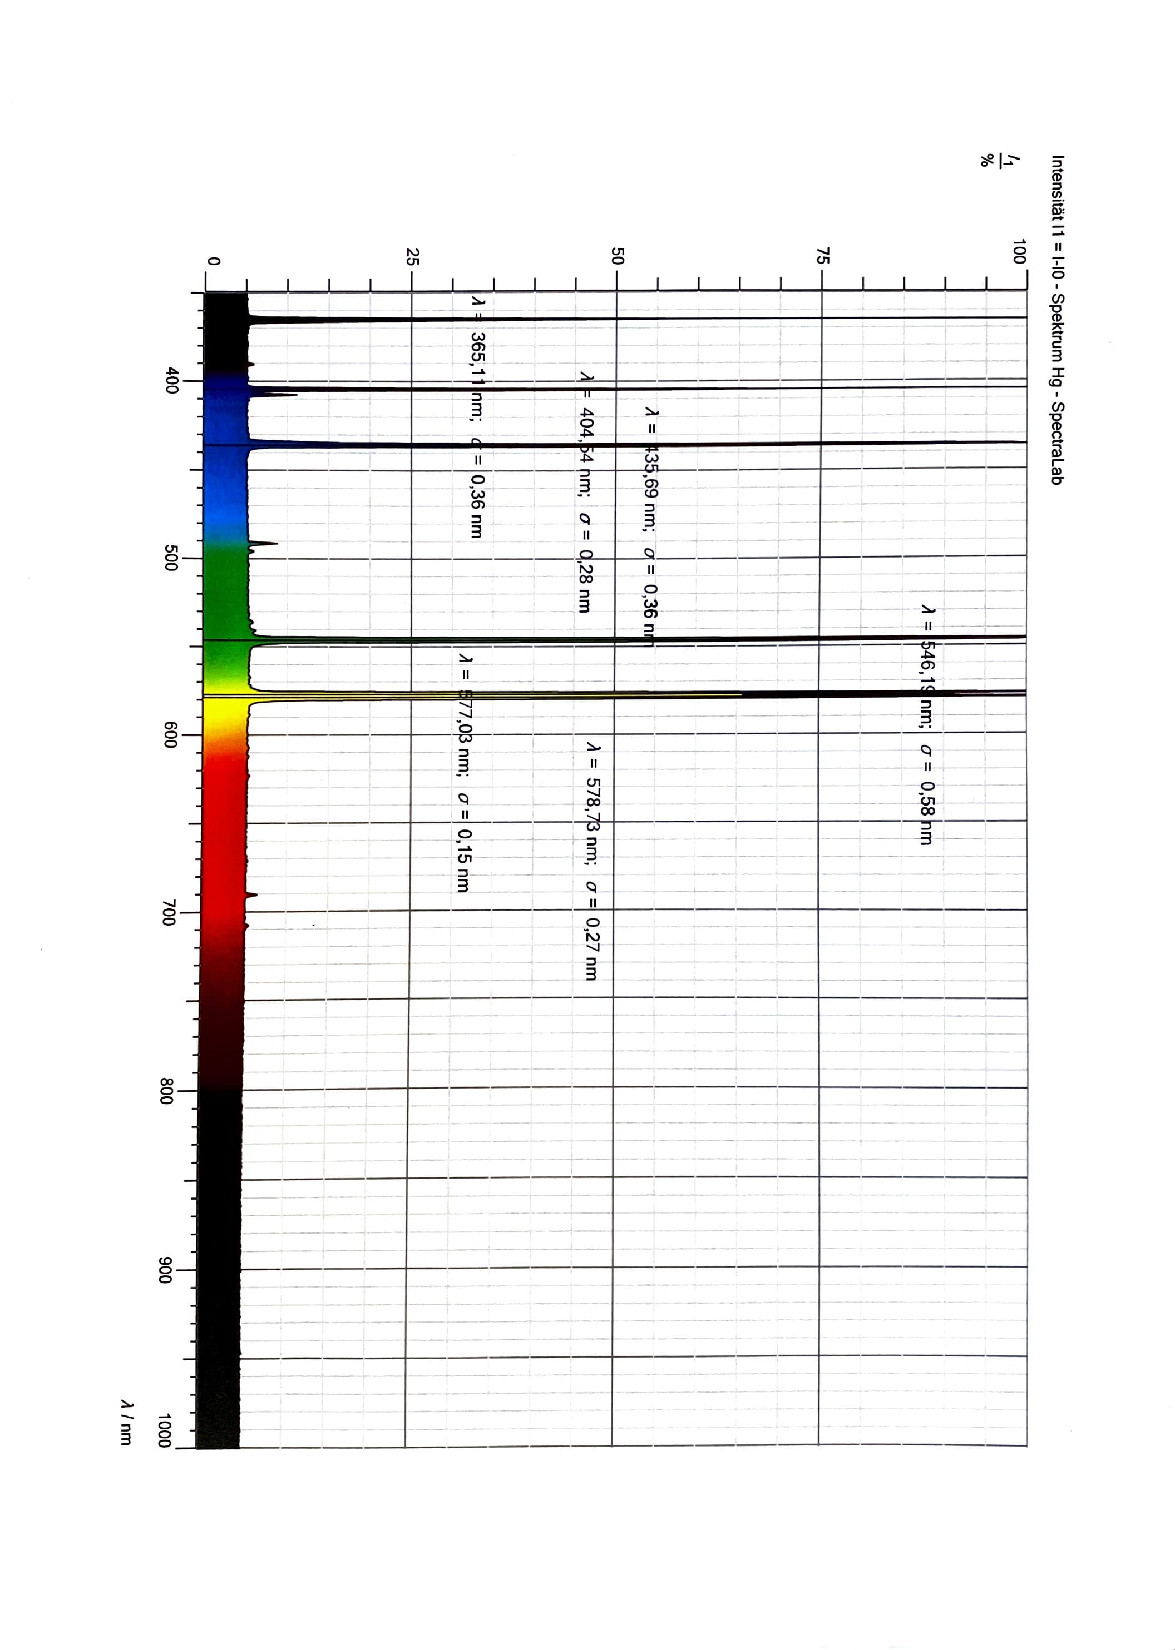
\includepdf[pages=-,scale=0.9,pagecommand={}]{PLW-Vorversuch.pdf}

\section{Anhang - Ausdrucke Teilversuch 1}
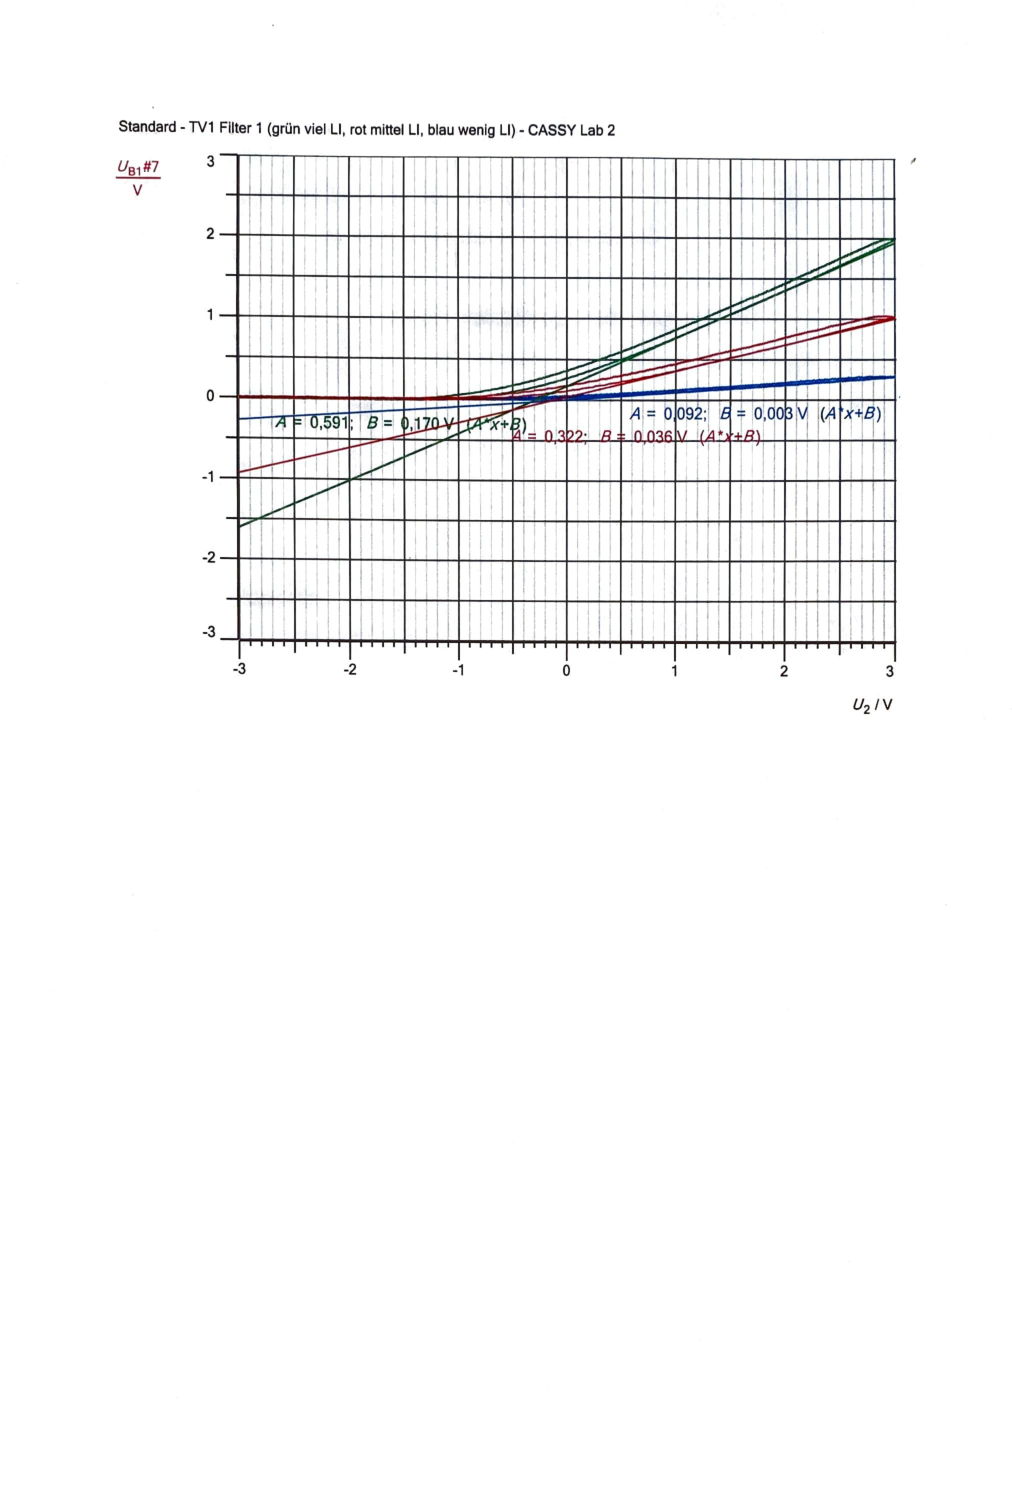
\includepdf[pages=-,scale=0.9,pagecommand={}]{PLW-TV1.pdf}

\section{Anhang - Ausdrucke Teilversuch 2}
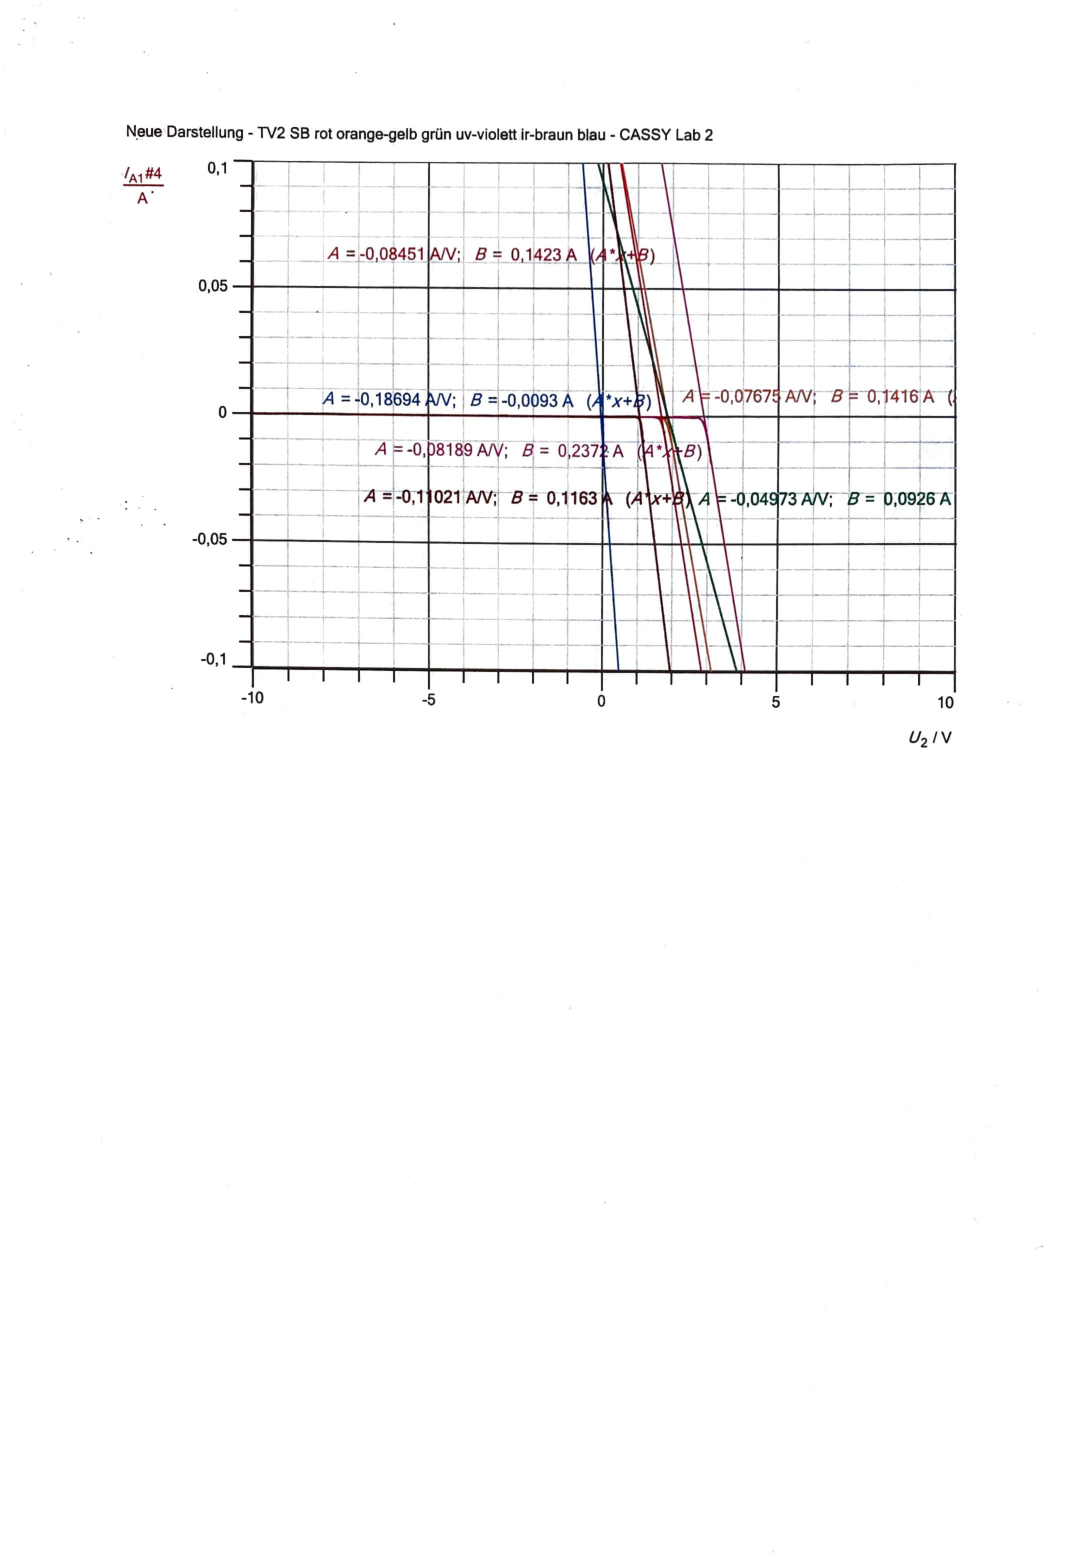
\includepdf[pages=-,scale=0.9,pagecommand={}]{PLW-TV2.pdf}


\section{Anhang --- Laborheft mit Testat}
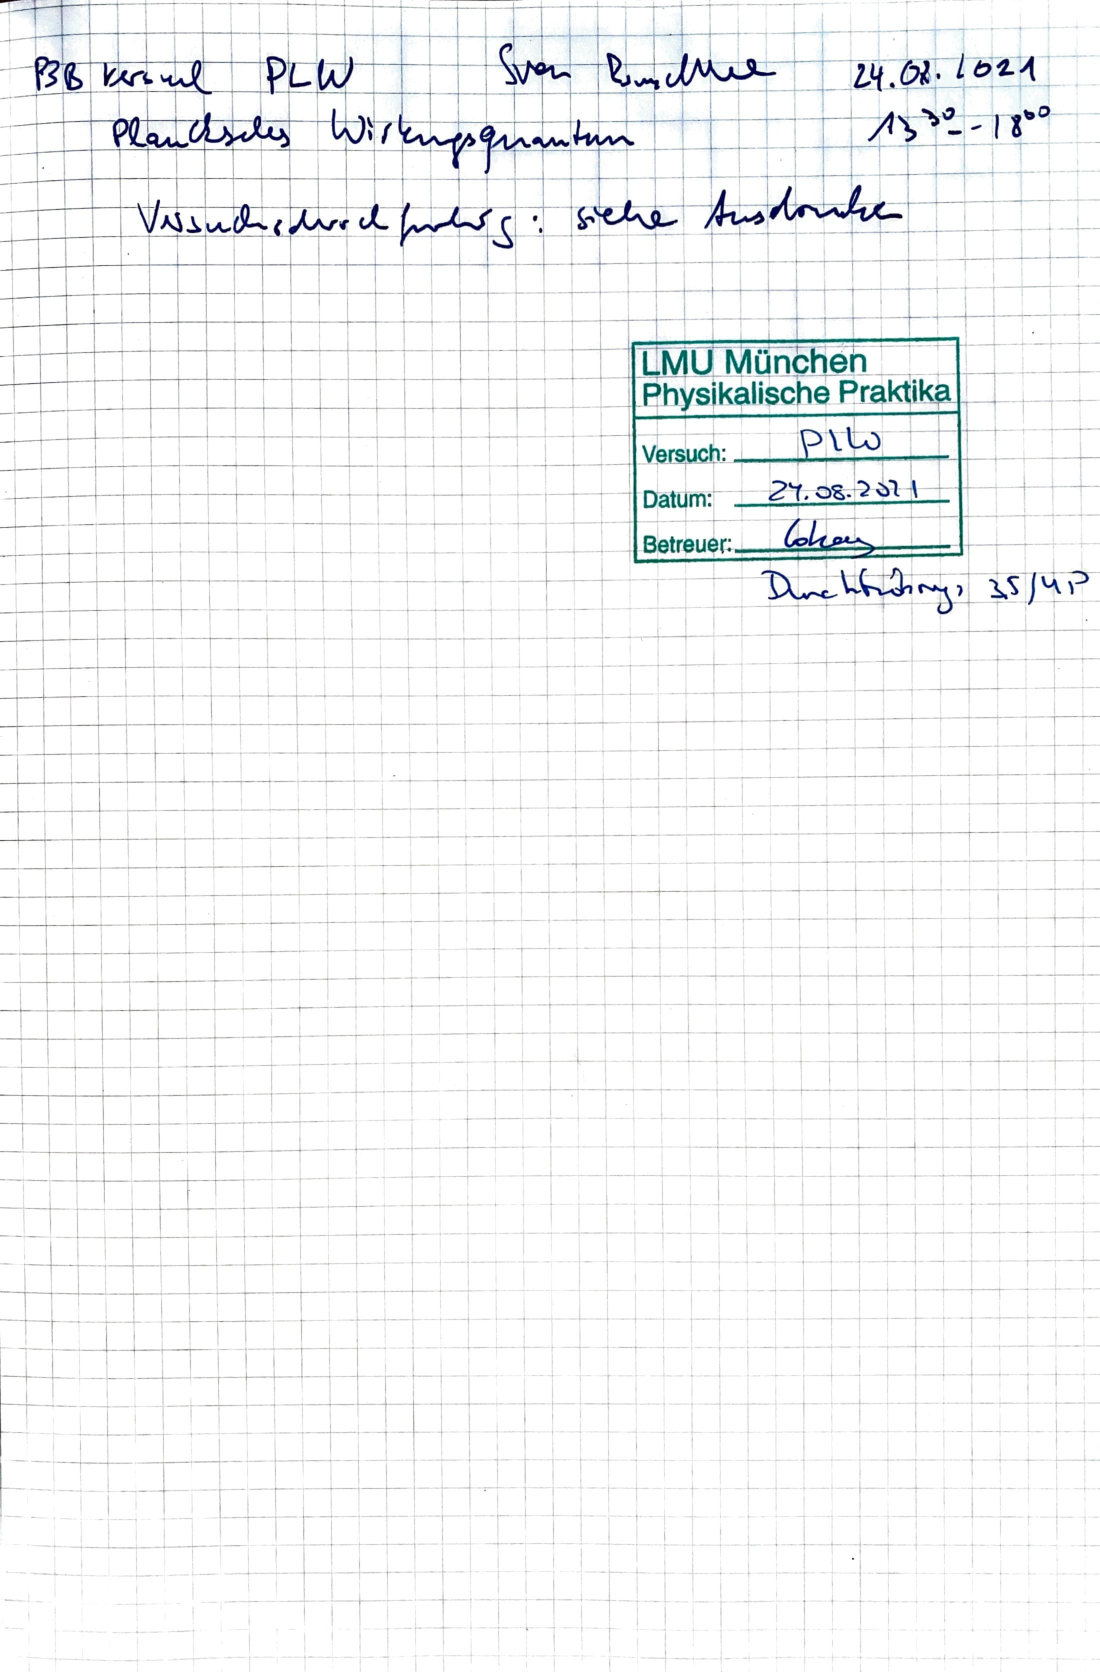
\includepdf[pages=-,scale=0.9,pagecommand={}]{PLW-Testat.pdf}

\end{document}